\documentclass[UTF8]{ctexart}
\usepackage{amsmath}
\usepackage{diagbox}
\usepackage{textcomp}
\usepackage{graphicx}
\usepackage{float}
\usepackage{caption}
\usepackage{adjustbox}
\usepackage{subfigure}
\usepackage{geometry}
\usepackage{pifont}
\usepackage{gensymb}
\usepackage{bm}
\usepackage{amstext}
\usepackage{amsfonts}
%引入代码块
\usepackage{listings}

\usepackage{xcolor}
%设置代码块格式

\definecolor{CPPGray}{RGB}{211,211,211}
\lstset{
 columns=fixed,       
 numbers=left,   % 在左侧显示行号
 numberstyle=\tiny\color{gray},% 设定行号格式
 frame=none,%none,% 不显示背景边框
 %aboveskip=1em,
 backgroundcolor=\color[RGB]{230,230,230},% 设定背景颜色
 keywordstyle=\color[RGB]{40,40,255},% 设定关键字颜色
 numberstyle=\footnotesize\color{darkgray},           
 commentstyle=\it\color[RGB]{0,96,96},% 设置代码注释的格式
 stringstyle=\rmfamily\slshape\color[RGB]{128,0,0},% 设置字符串格式
 showstringspaces=true,% 不显示字符串中的空格
 language=c++, % 设置语言
 morekeywords = {include,ull,int,double,return,static,typedef,if,else,for,long,void,class,struct,ll},                % 自加新的关键字(必须前后都是空格)
}

\begin{document}
\renewcommand{\thefootnote}{\fnsymbol{footnote}}
\newgeometry{left=2cm,bottom=3cm,right=2cm}
\linespread{1.4}
\title{\vspace{-5em}\heiti算法分析与设计基础\ \ 第二周作业\vspace{-2.5em}}
\date{}
\maketitle
\begin{center}
{\fangsong 徐浩博\quad 软件02\quad2020010108}
\end{center}


\subsection*{Problem 1}
\subsubsection*{a)}
$$T(n)=2T(\sqrt{n})+1$$令$2^m=n$,则有$$T(2^m)=2T(2^{m/2})+1$$
再令$S(m)=T(n)=T(2^m)$,则有$$S(m)=2S(m/2)+1$$
对照主定理的条件,$a=2,\ b=2$,则$m^{\log_b a}=n$,于是$f(m)=O(1)=O(m^{\log_b a-\epsilon})$,其中$\epsilon = 1$,根据定理有
$$S(m)=\Theta(m^{log_b a})=\Theta(m)$$
于是
$$T(n)=\Theta(log n)$$
\subsubsection*{b)}
$$nT(n)=(n-2)T(n-1)+2$$
则有$$n(n-1)T(n)=(n-1)(n-2)T(n-1)+2(n-1)$$
令$S(n)=n(n-1)T(n)$,则$$S(n)=S(n-1)+2(n-1)$$
于是有
\begin{align*}
    S(n)&=S(n-1)+2(n-1)\\ &=S(n-2)+2(n-2)+2(n-1)\\ & =\cdots\\
    & = 2\sum\limits^{n-1}_{i=1}i + S(1) \\ & = n(n-1) 
\end{align*}
则
\begin{align*}
    T(n)&=\frac{S(n)}{n(n-1)}=1=\Theta(1)
\end{align*}


\subsection*{Problem 2}
\section*{计算斐波那契数的方法比较实验报告}
\subsubsection*{摘要}
{\kaishu\normalsize  斐波那契数列可谓是世界上最为著名的数列之一,虽然可以通过数学方法找到通项公式,但在实际通过程序运算时,仍可能存在诸多问题. 本文介绍了编程计算斐波那契数的四种常见算法,并通过编写C++程序,对比各种算法的性能,包括计算结果误差和时间开销等. 通过对比,我们认为通项公式法实际上是一种编程上不太可行的算法,而通过矩阵乘法实现的logn复杂度的算法可以作为实际计算斐波那契数的一种理想的方法.}
\subsubsection*{关键词:斐波那契数列\ \ 通项公式\ \ 时间复杂度\ \ 空间复杂度\ \ 快速幂\vspace{1.5em}}

\section*{1\ \ \ 实验环境}
操作系统:Windows 10\par
IDE:Visual Studio 2019\par
处理器:Intel Core i7-10750H 六核CPU @ 2.60GHz\par
编程语言:C++11

\section*{2\ \ \ 算法分析}
\subsection*{2.1\ 暴力递归}
\paragraph{算法原理}\ \par
我们将函数原型写作\textbf{ull fiboBrute(ull n)},运用递归的方法计算斐波那契数列每一项的值. 具体来说,我们在函数内部递归调用fiboBrute(n - 1)与fiboBrute(n - 2)并将二者即可,代码如下:

\begin{lstlisting}
    ull fiboBrutal(ull n)
    {
        if (n <= 2) return 1;
        return fiboBrutal(n - 1) + fiboBrutal(n - 2);
    }
\end{lstlisting}

\paragraph{时间复杂度}\ \par
\begin{equation}T(n)=T(n-1)+T(n-2)\end{equation}
我们边界条件为$T(1)=T(2)=1$,由递推公式,我们可以看出
\begin{equation}T(n)=Fib(n)=\Theta(Fib(n))\end{equation}
而斐波那契数列的通项公式为指数函数,故该种算法具有指数级的时间复杂度.
\paragraph{空间复杂度}\ \par
栈深度为$\Theta(n)$,故算法空间复杂度$\Theta(n)$.

\subsection*{2.2\ 循环递推}
\paragraph{算法原理}\ \\
这种方法也易于理解,即通过递推公式从小到大向上递推,具体实现时可以借助一个for循环,如下:
\begin{lstlisting}
    ull a = 1, b = 1;
	for (ull i = 3; i <= n; i++)
	{
		b += a;
		a = b - a;
	}
\end{lstlisting}

\paragraph{时间复杂度}\ \par
循环进行了(n-2)次,每次循环都进行常数次运算,因此时间复杂度$\Theta(n)$.
\paragraph{空间复杂度}\ \par
程序只声明了常数个临时变量,空间复杂度为$\Theta(1)$.

\subsection*{2.3\ 通项公式计算}
\paragraph{算法原理}\ \par
斐波那契数列通项公式为\begin{equation}Fib(n)=\frac{1}{\sqrt{5}}((\frac{1+\sqrt{5}}{2})^n-(\frac{1-\sqrt{5}}{2})^n)\end{equation}\par
涉及浮点数运算,故我们均使用double进行计算. 计算某实数的n次幂时,我们采用快速幂的算法,具体说来,计算$c^n$的方法如下:
\begin{equation}c^n=c^{(a_m a_{m-1}\cdots a_{0})_2}=\prod\limits_{k=0}^m{c^{2^k\cdot a_k}}\label{kuaisumi}\end{equation}
因此我们将n按照二进制位展开,从低位到高位扫过一遍;在计算$2^k$的同时将结果连乘出来. 最后结果取四舍五入后转化为unsigned long long格式,具体代码见下:
\begin{lstlisting}
	const double sqrt5 = 2.23606797749978969641;
	double phi1 = (1 + sqrt5) / 2;
	double phi2 = (1 - sqrt5) / 2;
	double term1 = 1.;
	double term2 = 1.;

	while (n)
	{
		if (n & 1) term1 *= phi1, term2 *= phi2;
		phi1 *= phi1;
		phi2 *= phi2;
		n >>= 1;
	}
	return ull(round(term1 / sqrt5 - term2 / sqrt5));
\end{lstlisting}
\paragraph{时间复杂度}\ \par
由于n的二进制有logn位,因此从二进制低位到高位循环一遍,运算步骤为$clogn(c\in \mathbb{R})$,最终时间复杂度为$\Theta(logn)$.\par
\paragraph{空间复杂度}\ \par
程序只声明了常数个临时变量,空间复杂度为$\Theta(1)$.
\paragraph{递推写法变种}\ \par

事实上这种方法也可以递归实现:$c^n=c^{n/2}\cdot c^{n/2}$,时间复杂度递推式可以写作
\begin{equation}T(n)=T(n/2)+\Theta(1)\end{equation}\par
根据主定理,$a=1, b=2$,$n^{\log_ba}=1=\Theta(1)$,所以算法时间复杂度也为$\Theta(n)$,但空间复杂度为栈空间$\Theta(logn)$,比非递归写法略大.

\subsection*{2.4\ 矩阵法计算}
\paragraph{算法原理}\ \par
我们对矩阵
$E=\begin{bmatrix}1&1\\1&0\end{bmatrix}$
研究可以发现,若数列有$a_n=a_{n-1}+a_{n-2}$,那么$$
\begin{bmatrix}a_n\\a_{n-1}\end{bmatrix}=
\begin{bmatrix}1&1\\1&0\end{bmatrix}^n\begin{bmatrix}a_1\\a_0\end{bmatrix}$$
在这里$a_0=0,\ a_1=1$,故只需计算矩阵幂$E^n$即可得到结果. 计算矩阵幂时我们与(\ref{kuaisumi})式类似,只需将实数乘法修改为矩阵乘法即可,因此代码可以写成如下形式:

\begin{lstlisting}
	ull a[2][2]{ {1,0},{0,1} };
	ull pow[2][2]{ {1,1},{1,0} };
	while (n)
	{
		if (n & 1)	matrixMul(a, pow);
		matrixMul(pow, pow);
		n >>= 1;
	}
	return a[1][0];
\end{lstlisting}

\paragraph{时间复杂度}\ \par
与2.3分析类似,运算步骤为$clogn(c\in \mathbb{R})$,最终时间复杂度为$\Theta(logn)$.\\

\paragraph{空间复杂度}\ \par
程序只声明了常数个临时变量,空间复杂度为$\Theta(1)$.
\paragraph{递推写法变种}\ \par
与2.3的递推写法类似,
2.4的方法也可以用递归实现:$E^n=E^{n/2}\cdot E^{n/2}$,算法时间复杂度也为$\Theta(n)$,空间复杂度为栈空间$\Theta(logn)$,大于非递归写法.

\section*{3\ \ \ 结果分析}
\subsection*{3.1\ 误差分析}
对于2.3采用通项公式计算的方法,由于运用了浮点数运算,因此我们需要对其计算的误差进行分析. 然而,细致讨论算法中的浮点误差是困难的,因此我们作出如下假设:假设误差是由于计算$\phi_1^n$时浮点数小数位数有限造成的(在这里,$|\phi_2|<1$,$\lim\limits_{n\rightarrow \inf}\phi_2=0$忽略影响),假设double的浮点数保存时与真实值偏差为$d\phi$,那么有
$$(\phi+d\phi)^n\approx \phi^n + n\phi^{n-1}d\phi$$\par
误差即为$\Delta _{RESULT} = n\phi^{n-1}d\phi/\sqrt{5}\approx n Fib(n) d\phi$\par
我们假设double的精度误差为$d\phi = 10^{-15}$,事实上,$n=70$时,Fib(n)数量级达到$10^{14}$,因此$\Delta _{RESULT}$数量级就达到了$10^0-10^1$,可以从实验结果上看到显著偏差了. 下面的实验也证实了我们的猜想:
下面我们将进行实验,我们将实验的n控制在$70-90$附近的区间(n过大时。double类型变量可能会自然溢出),并得出下列实验结果. \textbf{注意,以下结果均已对1e9+7取模}:

\begin{table}[H]
	\begin{center}
    \centering{\caption{采用浮点数方法计算的结果与真实值的对比}}
		\begin{tabular}{c|c|c|c}
			\hline
			n&数列第n项真实值&通项公式法计算结果&误差\\
			\hline
			\hline
			69 & 29637311 & 29637311 & 0\\
			\hline
			72 & 8390086 & 8390086 & 0\\
			\hline
			75 & 63197655 & 63197655 & 0\\
			\hline
			78 & 261180706 & 261180705 & 1\\
			\hline
			81 & 107920472 & 107920462 & 10\\
			\hline
			84 & 692862594 & 692862546 & 48\\
			\hline
			87 & 879370834 & 879370672 & 162\\
			\hline
			90 & 210345902 & 210345270 & 632\\
			\hline
		\end{tabular}
\end{center}\end{table}
可以看到,$n>75$时,计算值和真实值出现了偏差,这与我们的预测$n\approx 70$时出现偏差吻合得较好,说明我们的预测和实验结果均是正确的.

\subsection*{3.2\ 计算时间分析}
首先我们将四种方法放在一起进行比较;考虑到暴力递归法具有指数级的时间复杂度,故n不宜取大. 我们取n为$0-40$进行实验:
\begin{figure}[H]\begin{center}
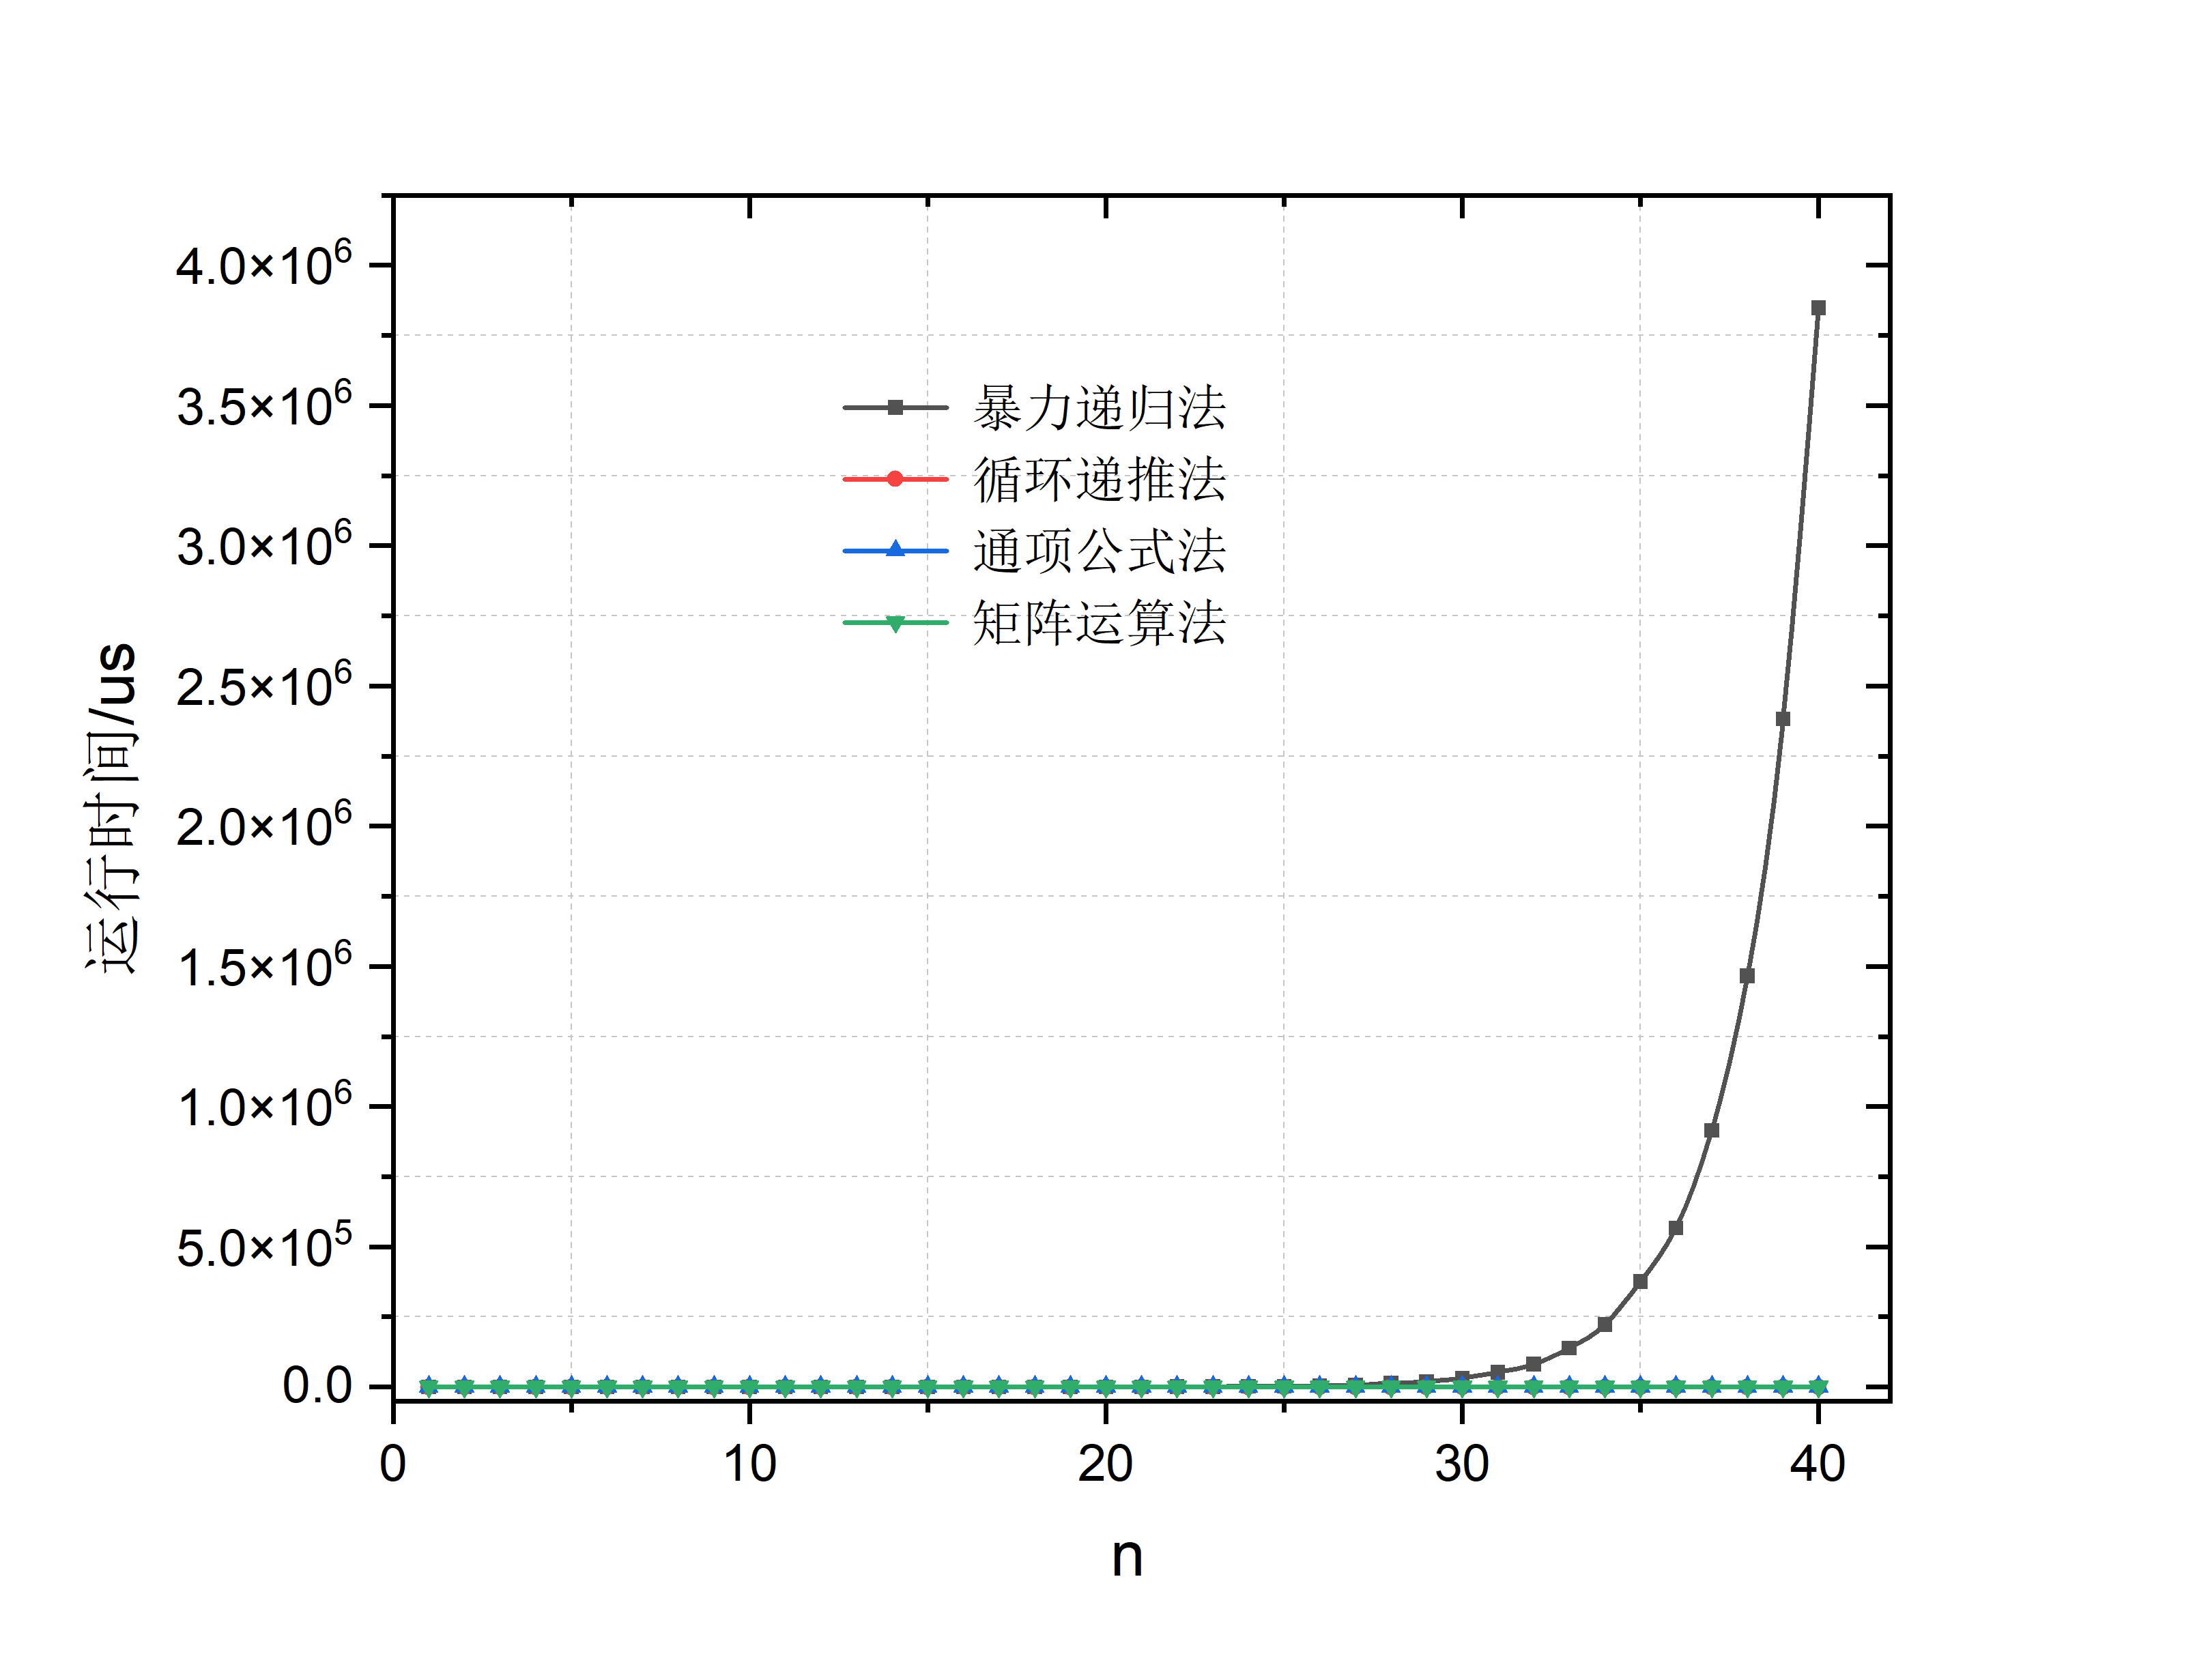
\includegraphics[scale = 0.5]{graph1.png}
\caption{四种计算方法运算时间对比图($n\in (0,40]$)}
\end{center}\end{figure}
从中我们可以明显看出具有指数级复杂度的暴力递归法显著慢于其余三种(小于等于)多项式时间复杂度的方法.\par
进而,我们去除暴力递归法,对其余三种计算方法进行比较,得到如下结果:
\begin{figure}[H]\begin{center}
	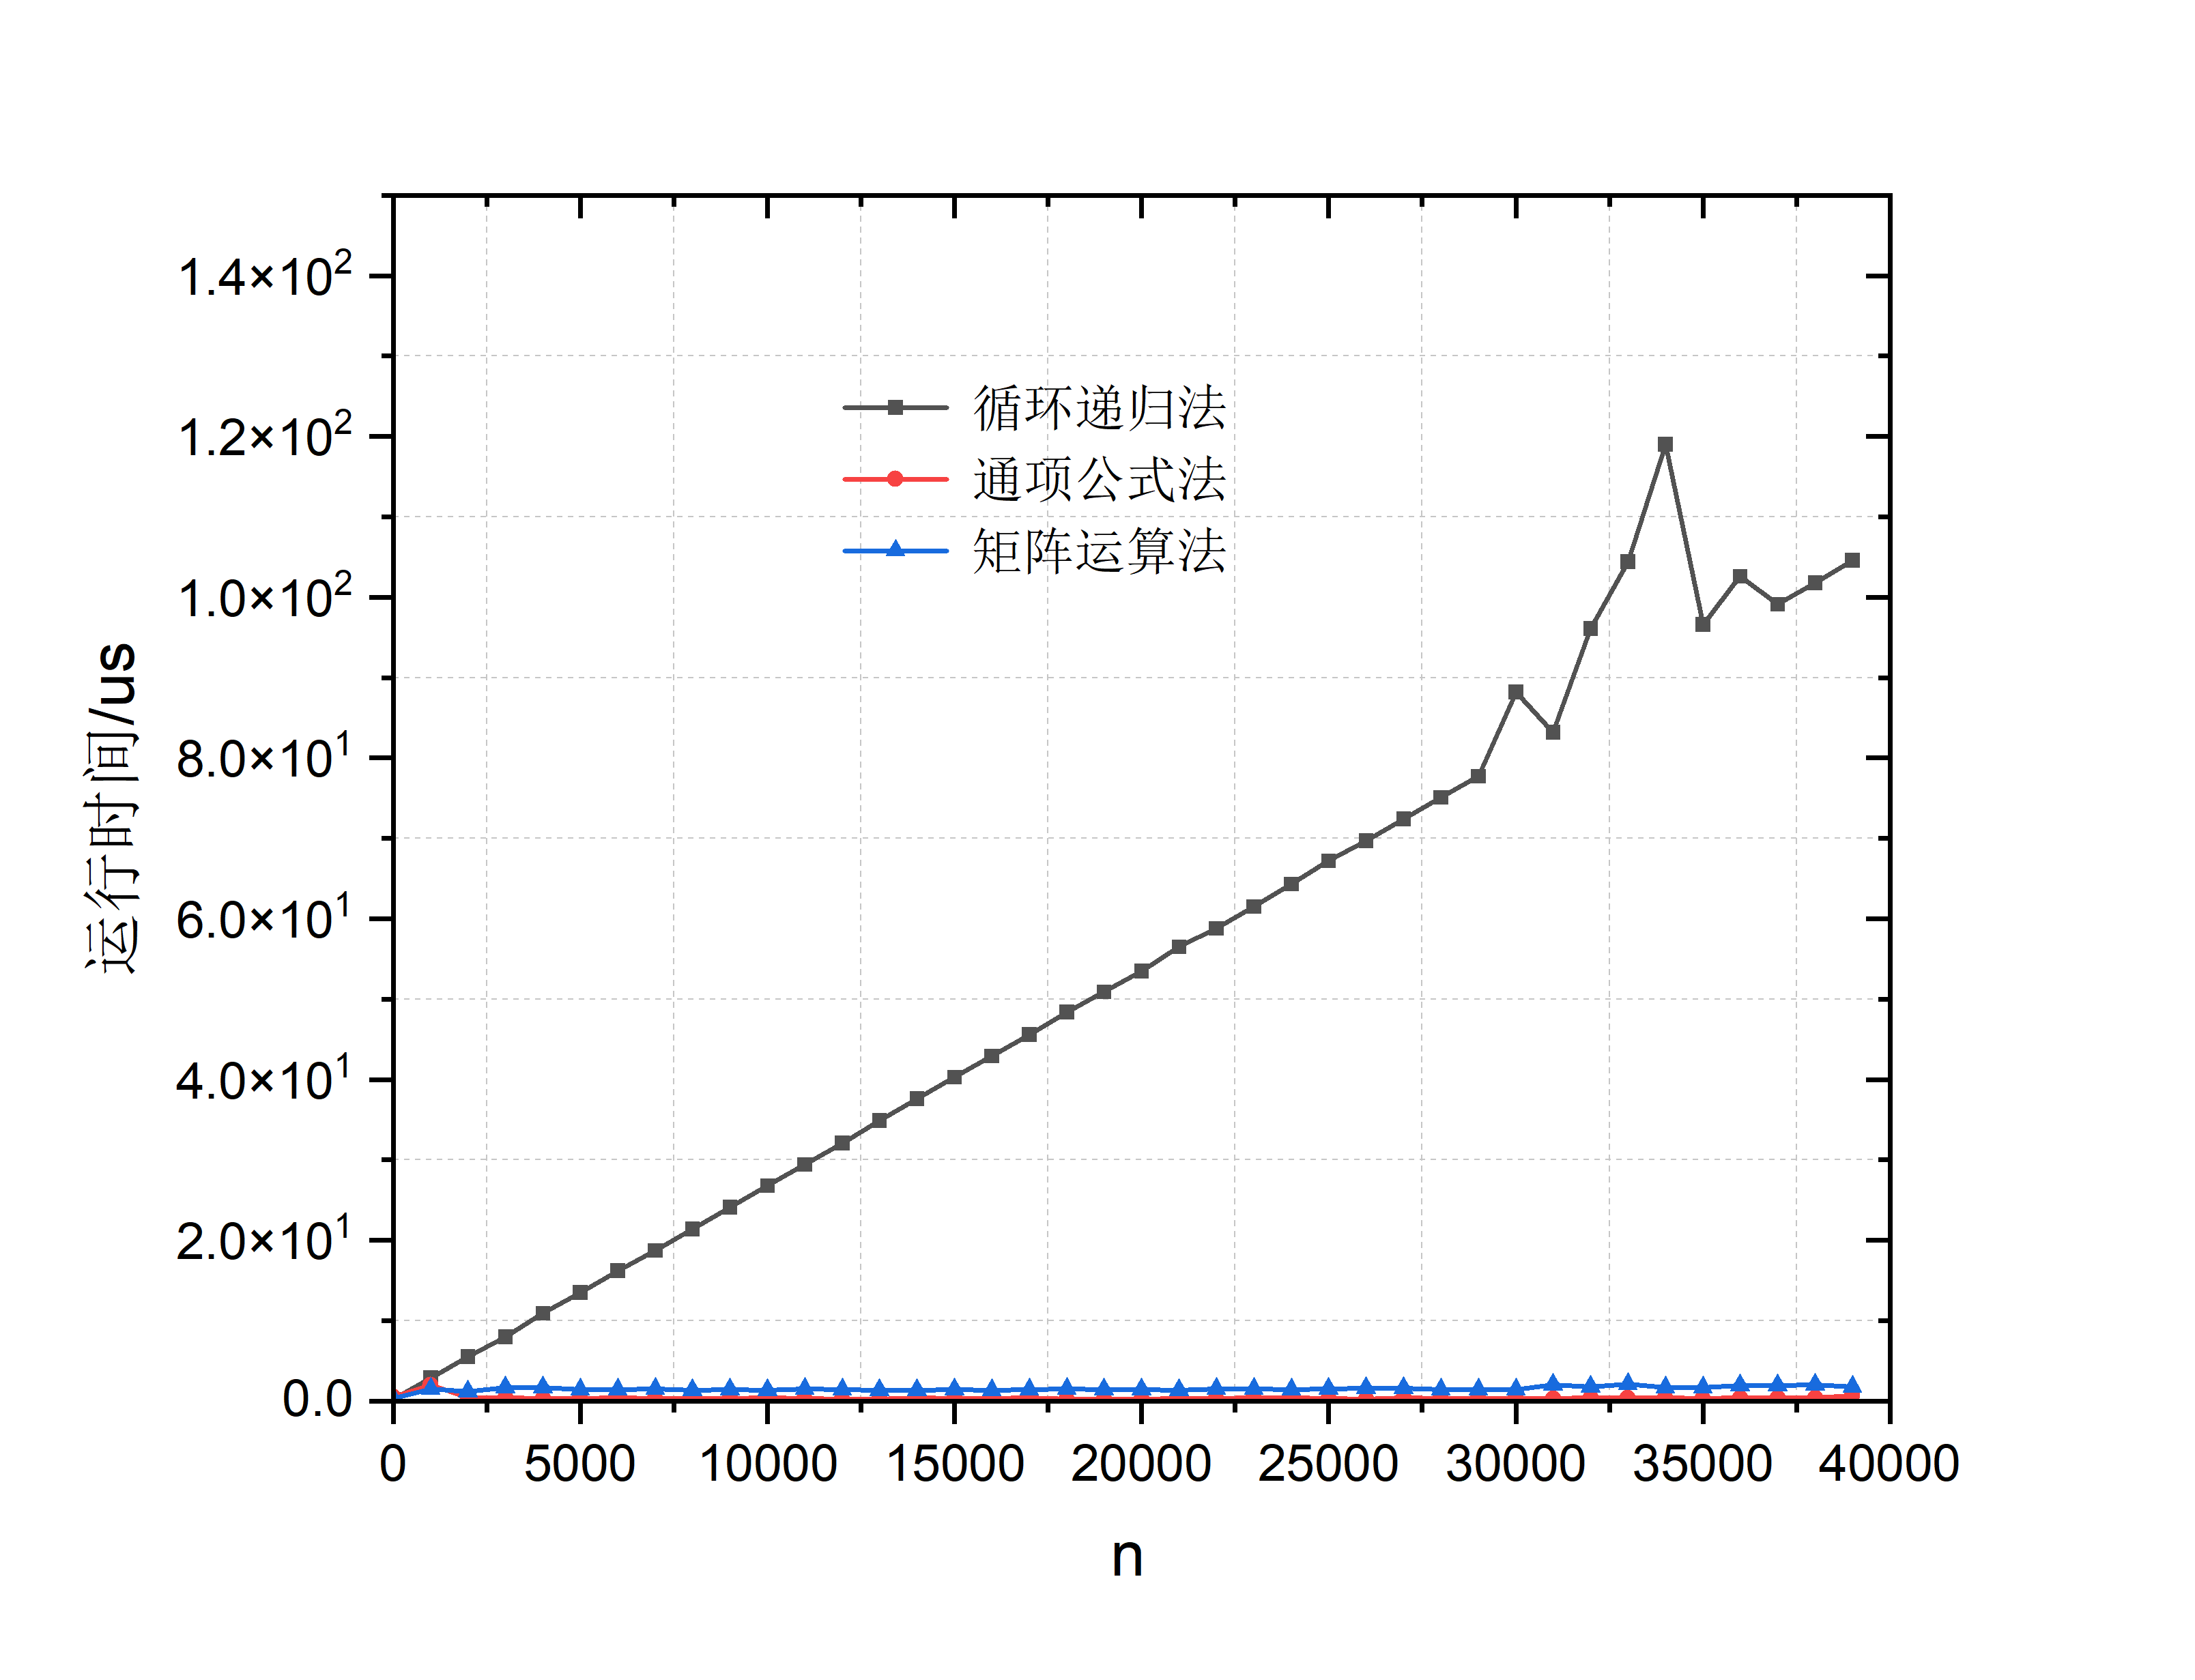
\includegraphics[scale = 0.5]{graph2.png}
	\caption{三种计算方法运算时间对比图($n\in (0,40000]$)}
\end{center}\end{figure}
可以看到,规模较大时,线性时间复杂度的循环递推法明显慢于其余两种具有对数级别时间复杂度的方法.\par
我们接着对这个图的初始部分进行放大,研究规模较小时的时间开销:
\begin{figure}[H]\begin{center}
	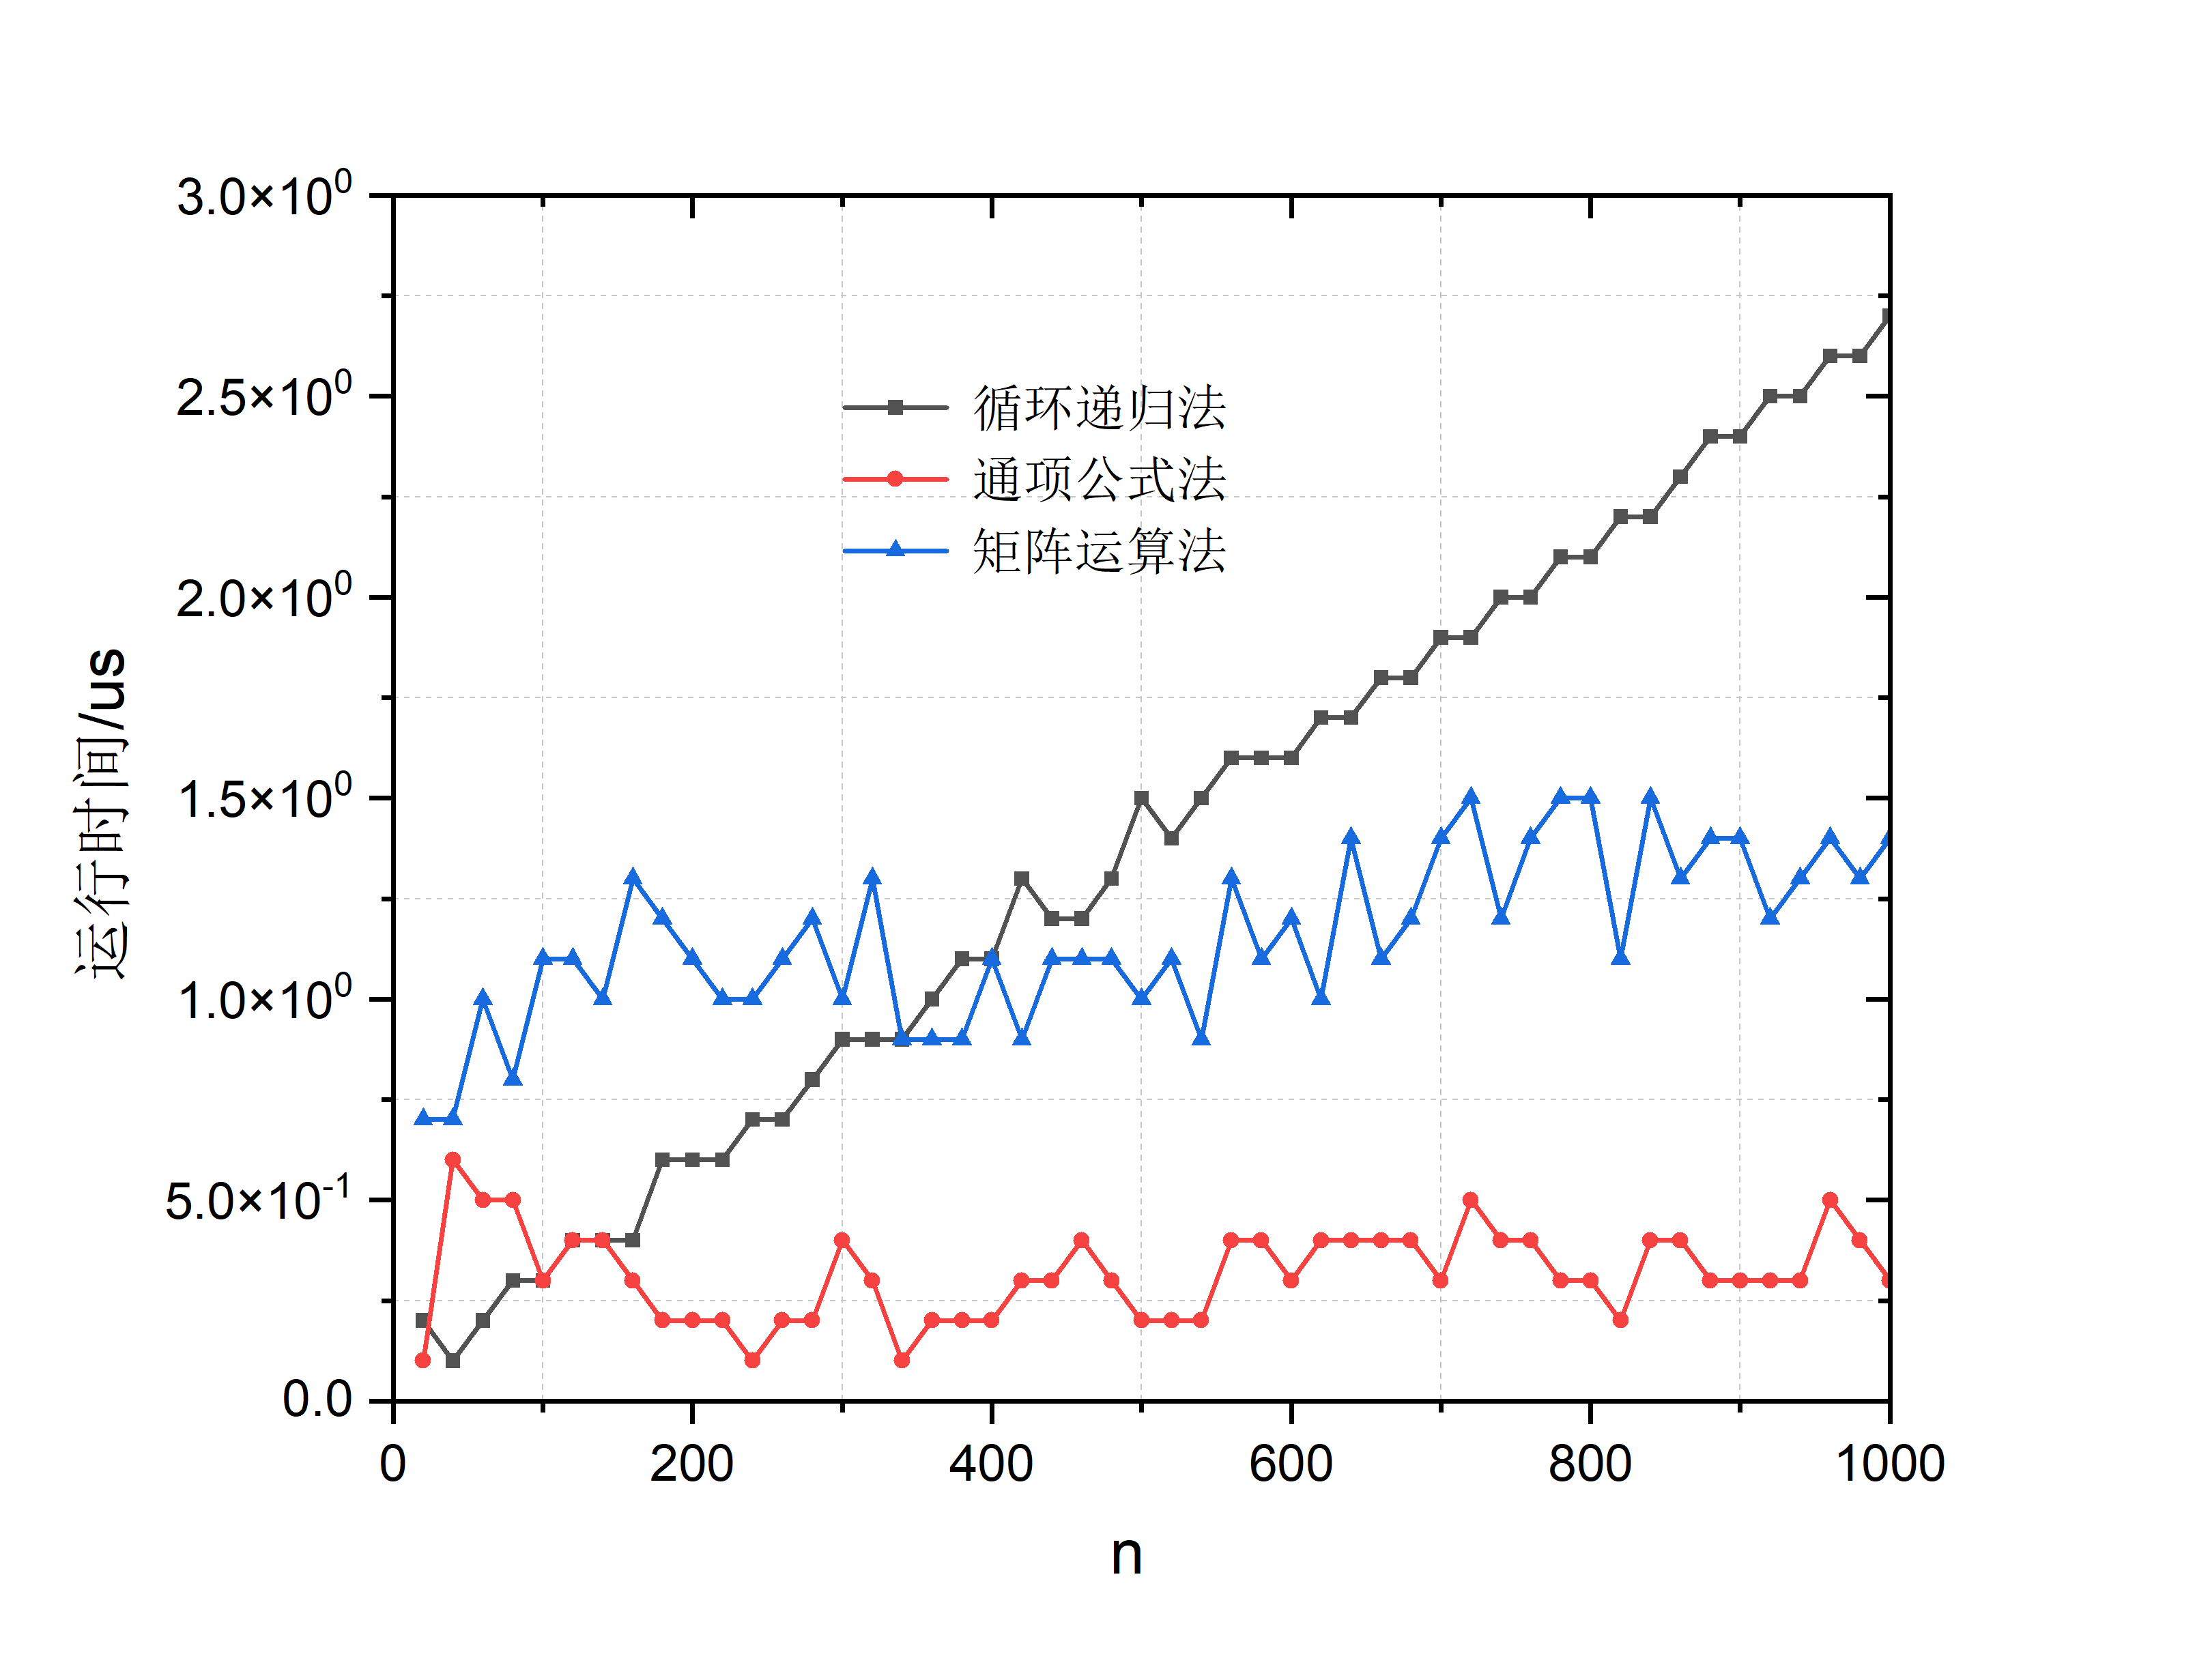
\includegraphics[scale = 0.5]{graph4.png}
	\caption{三种计算方法运算时间对比图($n\in (0,1000]$)}
\end{center}\end{figure}
可以看到,虽然通项公式法仍旧出色;但规模较小时(如n<300),循环递推法快于矩阵运算法,这可能与矩阵运算的时间复杂度具有较大的常数因子有关. 但随着规模扩大,循环递推法线性增长,而矩阵运算法较为稳定,几乎看不到增长趋势,因此很快,循环递推法就远差于矩阵运算法了.\par
在这里,我们再次去除循环递推法,扩大n的范围,对通项公式法和矩阵运算法再进行比较:
\begin{figure}[H]\begin{center}
	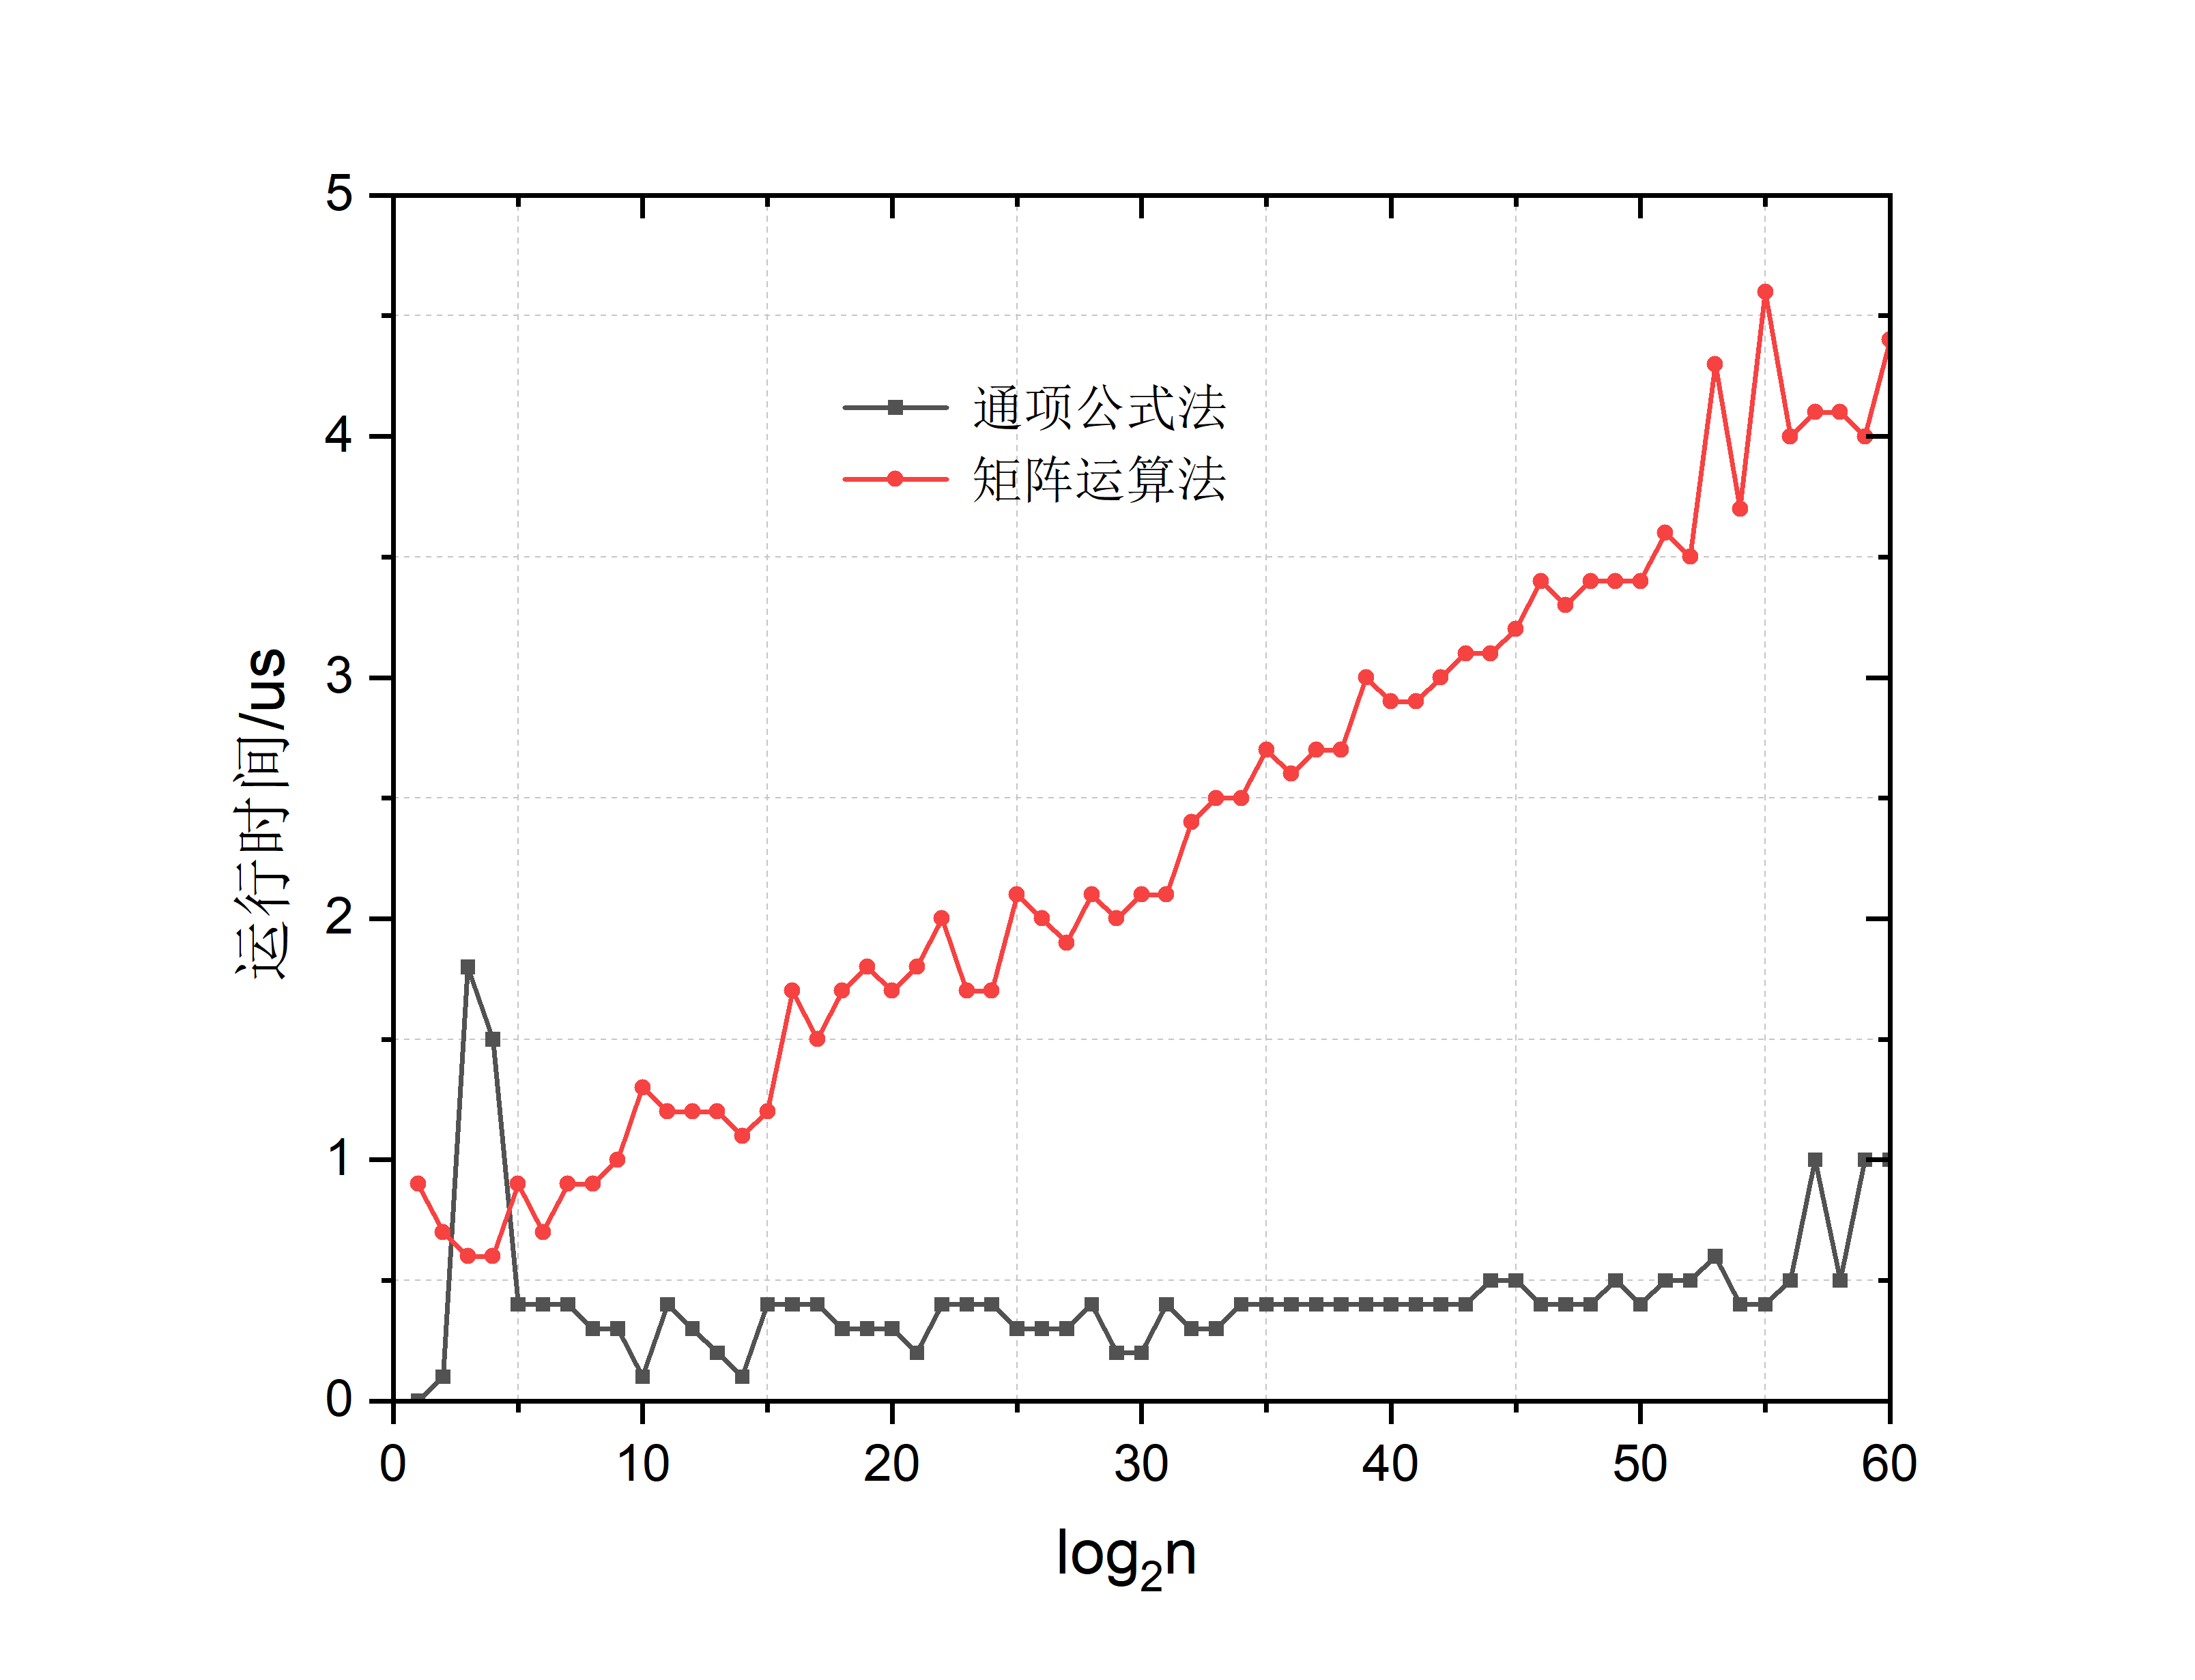
\includegraphics[scale = 0.5]{graph3.png}
	\caption{通项公式法和矩阵运算法运算时间对比图($n\in (0,2^{60}]$)}
\end{center}\end{figure}
我们能从图像看出来,虽然通项公式法和矩阵运算法具有相同的时间复杂度,但实际运行时,前者的常数要小于后者. 实际上我们会看到,n值非常大的某项求值似乎并没有多大用处;实际应用中,矩阵运算法的速度是足以满足需求的.\par
在这里我们还需要强调一点,虽然我们在3.1部分看到,通项公式法由于涉及浮点运算,可能产生较大的误差;但事实上,由于计算结果过于庞大,欲得出正确的结论,我们使用矩阵运算法时,也需要使用高精度运算;这也是想要使用通项公式法得出正确结论所必须的. 从这个角度上来看,矩阵运算法的表现或许也没有那么糟糕.

\section*{4\ \ \ 总结}
根据以上分析,我们将四种方法总结如下:
\paragraph{暴力递归} 时间复杂度高,需要使用栈;面对大规模的数据,无论是时间开销抑或是栈空间开销,均是无法承受的.
\paragraph{循环递归} 线性时间复杂度,写法简单. 面对小规模数据(1e2量级),性能甚至可能优于对数级别时间复杂度的算法;但大规模数据计算的时间开销仍较大.
\paragraph{通项公式} 对数级别时间复杂度,且对数的常数较小,运算速度是几种方法中最快的,然而考虑到用c++语言实现时,在n=70左右就会因浮点数计算而出现明显误差,且n=100左右double会溢出,所以只能作为一种理论可行但实际上几乎不会采取的办法.
\paragraph{矩阵运算} 对数级别时间复杂度,时间开销较小,面对大规模数据也能从容不迫,适合于处理n较大且对性能要求较高的场合.
\end{document}
